% Provenance (never printed): cycle 3 "La planete Terre" (natural phenomena
% and the risks they bring: storms, floods, droughts, earthquakes, eruptions;
% warnings and the right behaviour); see sources/book1/PROVENANCE.md.
% Book 1, grade 5, chapter 3.
\chapter{As ameaças naturais}\label{ch:g5:natural-hazards}

É sexta-feira à noite. No rádio, a música para e uma voz calma lê um
alerta: uma \omterm{def:g5:natural-hazards:storm}{tempestade} forte vai chegar ao \omterm{def:g1:landscapes-around-us:water}{litoral} esta noite, com ventos
muito fortes e \omterm{def:g4:clouds-rain-snow:precipitation}{chuva} forte. Pede-se às pessoas que fiquem dentro de casa a
partir das nove horas e que amarrem ou guardem tudo o que o vento possa
levar.

A família de Lena começa a trabalhar. O pai guarda as cadeiras e a mesa do
jardim no depósito. A mãe confere se as lanternas funcionam e põe pilhas
de reserva na mesa da cozinha. Lena enche duas garrafas grandes de água.
Às nove horas, todos estão dentro de casa, e o vento já está uivando.

\begin{omfigure}

\includegraphics[width=0.5\linewidth]{images/book1/ai/g5-radio-warning.jpg}

{\small Uma família ouve um alerta de \omterm{def:g5:natural-hazards:storm}{tempestade} no rádio, com lanternas e
pilhas de reserva à mão.}
\end{omfigure}

\begin{recall}
Um \omterm{def:g4:volcanoes-earthquakes-first-look:volcano}{vulcão} pode entrar em \omterm{def:g4:volcanoes-earthquakes-first-look:eruption}{erupção}, lançando \omterm{def:g4:volcanoes-earthquakes-first-look:eruption}{lava}, cinza e gases; um
\omterm{def:g4:volcanoes-earthquakes-first-look:earthquake}{terremoto} é um tremor repentino do chão; num \omterm{def:g4:volcanoes-earthquakes-first-look:earthquake}{terremoto}, nós nos abaixamos,
nos protegemos e nos seguramos (\cref{ch:g4:volcanoes-earthquakes-first-look}).
Um \omterm{def:g1:landscapes-around-us:water}{rio} que recebe mais água do que o seu canal consegue conter inunda a
sua \omterm{def:g5:water-shapes-the-land:flood}{planície de inundação} (\cref{ch:g5:water-shapes-the-land}). Cada lugar
tem o seu \omterm{def:g5:weather-and-climate:climate}{clima}, e as zonas quente, temperadas e frias dão a volta no
\omterm{def:g3:continents-and-oceans:globe}{globo} (\cref{ch:g5:weather-and-climate}).
\end{recall}

\section{O que é uma ameaça natural}

A natureza nem sempre é calma. O vento pode soprar forte o bastante para
quebrar árvores, os \omterm{def:g1:landscapes-around-us:water}{rios} podem transbordar, o chão pode tremer. Esses
acontecimentos fazem parte do funcionamento da Terra: eles aconteciam
muito antes de existirem pessoas, e vão continuar acontecendo.

\begin{definition}[Ameaça natural]\label{def:g5:natural-hazards:hazard}
Uma \emph{ameaça natural}\index{ameaca natural@ameaça natural} é um acontecimento natural que
pode ferir as pessoas ou danificar o que elas construíram: uma \omterm{def:g5:natural-hazards:storm}{tempestade},
uma \omterm{def:g5:water-shapes-the-land:flood}{inundação}, uma \omterm{def:g5:natural-hazards:drought}{seca}, um \omterm{def:g4:volcanoes-earthquakes-first-look:earthquake}{terremoto}, uma \omterm{def:g4:volcanoes-earthquakes-first-look:eruption}{erupção} vulcânica, um
\omterm{def:g5:natural-hazards:landslide}{deslizamento de terra}{\ldots}
\end{definition}

Podemos classificar as \omterm{def:g5:natural-hazards:hazard}{ameaças naturais} pela sua origem: o ar, a água ou o
chão.

\begin{omfigure}
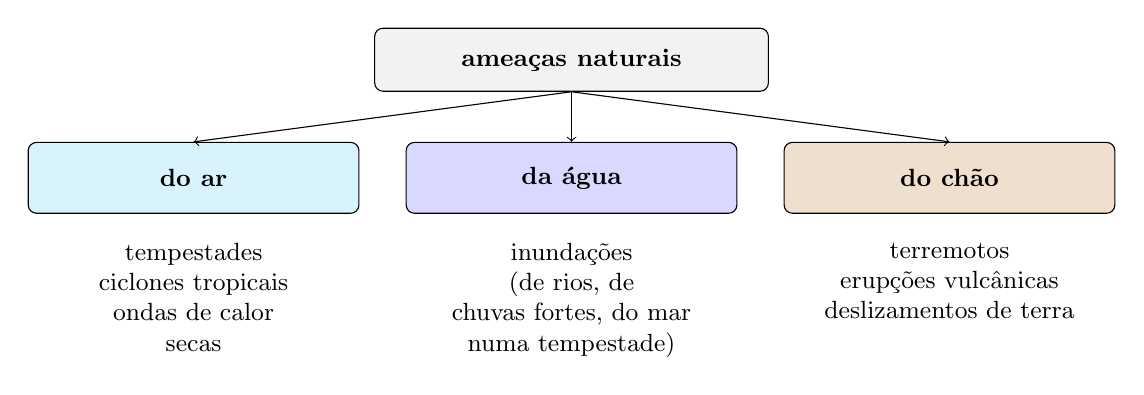
\begin{tikzpicture}[font=\small, box/.style={draw, rounded corners=3pt,
    minimum width=4.2cm, minimum height=0.9cm, align=center}]
  \node[box, fill=cyan!15, font=\small\bfseries] (A) at (0,0) {do ar};
  \node[box, fill=blue!15, font=\small\bfseries] (W) at (4.8,0) {da água};
  \node[box, fill=brown!25, font=\small\bfseries] (G) at (9.6,0) {do chão};
  \node[align=center, anchor=north] at (0,-0.7) {tempestades\\ciclones tropicais\\ondas de calor\\secas};
  \node[align=center, anchor=north] at (4.8,-0.7) {inundações\\(de rios, de\\chuvas fortes, do mar\\numa tempestade)};
  \node[align=center, anchor=north] at (9.6,-0.7) {terremotos\\erupções vulcânicas\\deslizamentos de terra};
  \node[draw, rounded corners=3pt, fill=gray!10, font=\small\bfseries,
    minimum width=5cm, minimum height=0.8cm] (N) at (4.8,1.5) {ameaças naturais};
  \draw[->] (N.south) -- (A.north);
  \draw[->] (N.south) -- (W.north);
  \draw[->] (N.south) -- (G.north);
\end{tikzpicture}

{\small As \omterm{def:g5:natural-hazards:hazard}{ameaças naturais}, classificadas pela sua origem.}
\end{omfigure}

\section{As ameaças que vêm do ar}

\begin{definition}[Tempestade]\label{def:g5:natural-hazards:storm}
Uma \emph{tempestade}\index{tempestade} é um período de vento muito forte,
em geral com \omterm{def:g4:clouds-rain-snow:precipitation}{chuva} forte ou \omterm{def:g4:clouds-rain-snow:precipitation}{neve}, e às vezes com trovões e raios.
\end{definition}

Uma \omterm{def:g5:natural-hazards:storm}{tempestade} forte quebra galhos, derruba árvores, arranca telhas dos
telhados e pode atirar cadeiras de jardim contra as janelas. No \omterm{def:g1:landscapes-around-us:water}{litoral}, o
seu vento empilha o \omterm{def:g2:water-on-earth:ocean}{mar} contra a costa e lança ondas enormes por cima dos
\omterm{def:g2:water-on-earth:ocean}{quebra-mares}.

As \omterm{def:g5:natural-hazards:storm}{tempestades} mais poderosas da Terra se formam sobre \omterm{def:g2:water-on-earth:ocean}{mares} tropicais
quentes. São \omterm{def:g5:natural-hazards:storm}{tempestades} enormes, que giram: vistas do espaço, elas
parecem uma espiral gigante de \omterm{def:g4:clouds-rain-snow:cloud}{nuvens}, com um buraco calmo e limpo no
meio, o olho. Em volta do olho sopram os ventos mais fortes. O mesmo tipo
de \omterm{def:g5:natural-hazards:storm}{tempestade} tem nomes diferentes em \omterm{def:g2:water-on-earth:ocean}{oceanos} diferentes: ele se chama
\emph{furacão} no Atlântico Norte e no leste do Pacífico, \emph{tufão} no
noroeste do Pacífico, e \emph{ciclone tropical} no Pacífico Sul e no
\omterm{def:g2:water-on-earth:ocean}{oceano} Índico.
% ledger: noaa:cyclone-names

\begin{omfigure}
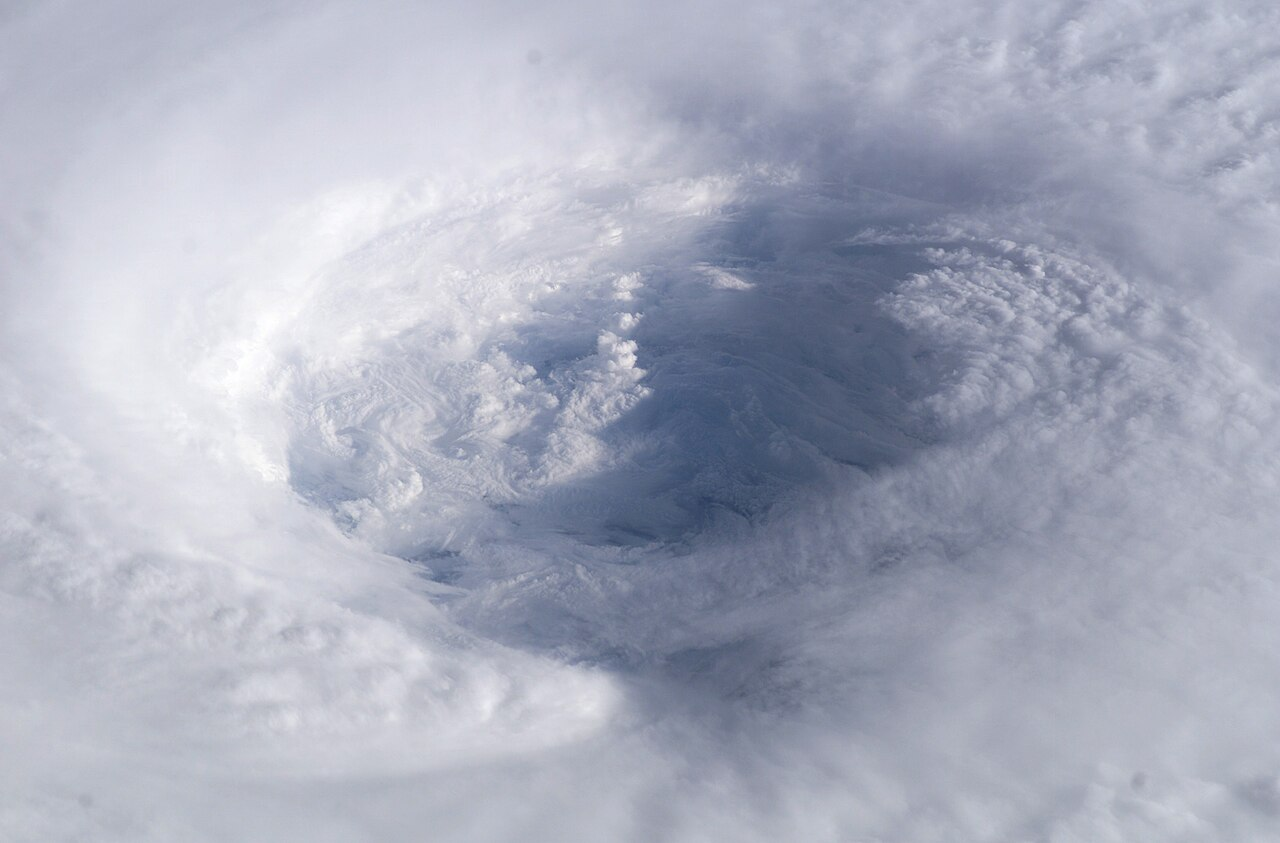
\includegraphics[width=0.5\linewidth]{images/book1/g5-hurricane-isabel-iss.jpg}

{\small O olho do furacão Isabel visto de cima, sobre o \omterm{def:g2:water-on-earth:ocean}{oceano} Atlântico,
em setembro de 2003, da Estação Espacial Internacional: uma parede de
\omterm{def:g4:clouds-rain-snow:cloud}{nuvens} em volta de um centro mais calmo. Foto: NASA (domínio público).}
% ledger: nasa:isabel-iss
\end{omfigure}

Algumas ameaças que vêm do ar são lentas e silenciosas. Uma \emph{onda de
calor} é um período de vários dias e noites muito mais quentes que o
normal. Ela é perigosa sobretudo para os idosos, os bebês e os doentes.

\begin{definition}[Seca]\label{def:g5:natural-hazards:drought}
Uma \emph{seca}\index{seca} é um período longo, de meses ou até de anos,
com muito menos \omterm{def:g4:clouds-rain-snow:precipitation}{chuva} que o normal para aquele lugar. O solo resseca, os
\omterm{def:g1:landscapes-around-us:water}{rios} e os \omterm{def:g1:landscapes-around-us:water}{lagos} encolhem, as plantações murcham e morrem.
\end{definition}

Uma \omterm{def:g5:natural-hazards:drought}{seca} chega devagar: ninguém sabe dizer em que dia ela começa. Mas uma
\omterm{def:g5:natural-hazards:drought}{seca} longa pode deixar os agricultores sem colheita e as cidades com falta
de água.

\begin{omfigure}
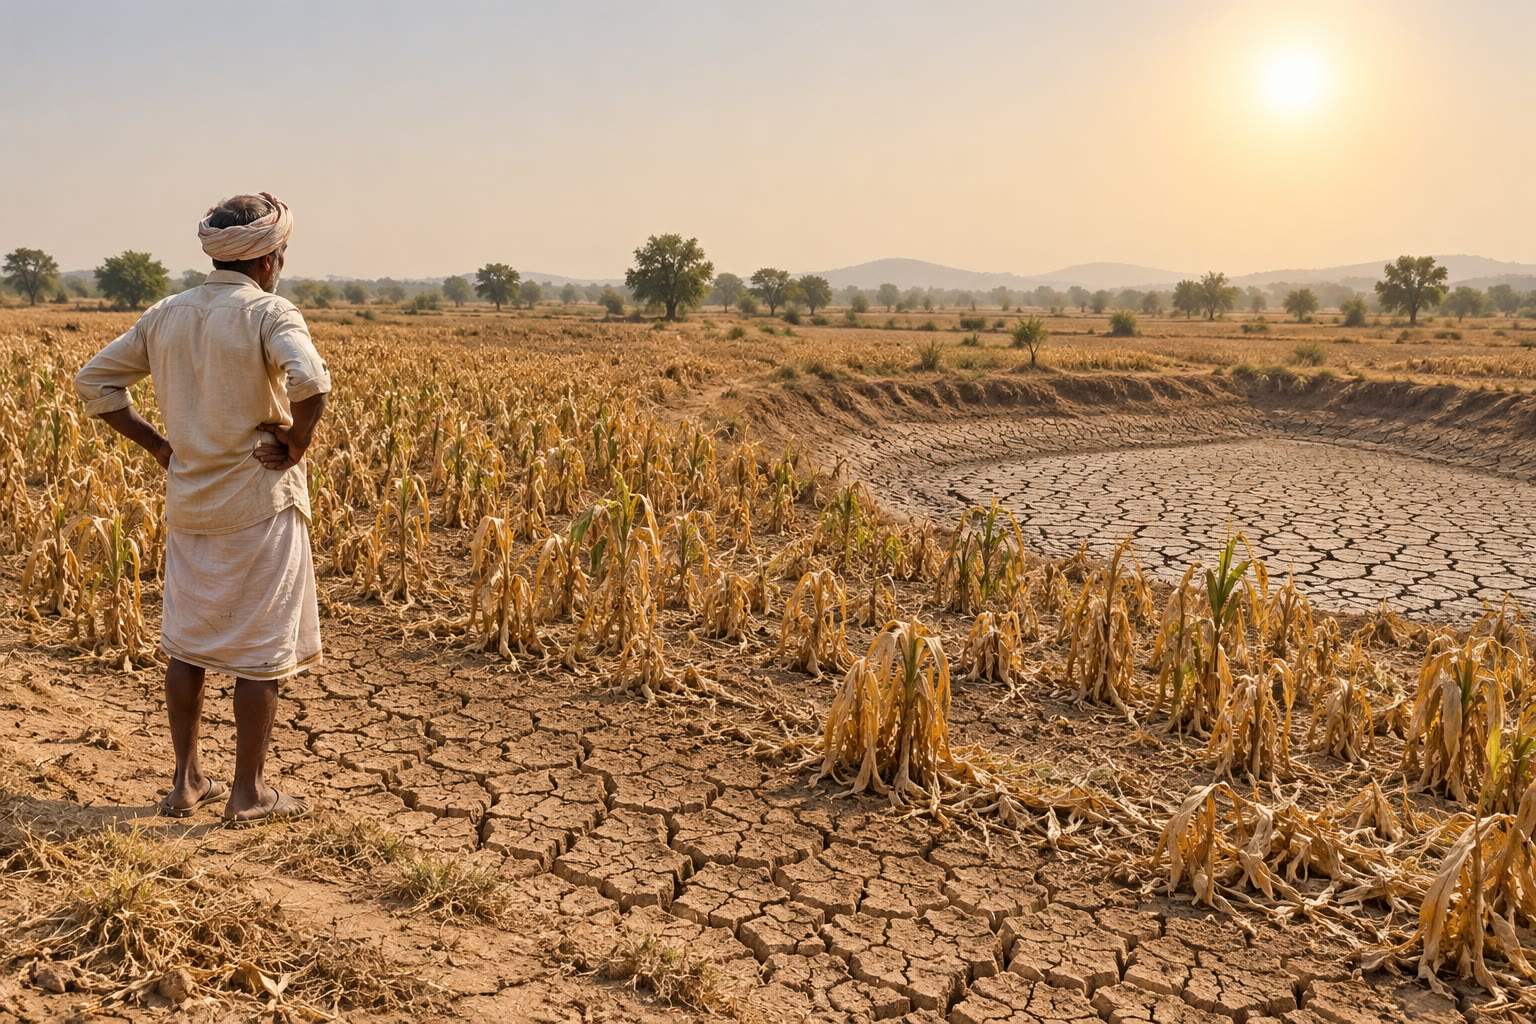
\includegraphics[width=0.42\linewidth]{images/book1/ai/g5-drought-field.jpg}

{\small Um campo numa \omterm{def:g5:natural-hazards:drought}{seca} longa: a terra está rachada, as plantações estão
amarelas e o açude secou.}
\end{omfigure}

\section{As ameaças que vêm da água}

Você já conhece as \omterm{def:g5:water-shapes-the-land:flood}{inundações} dos \omterm{def:g1:landscapes-around-us:water}{rios} (\cref{ch:g5:water-shapes-the-land}).
Depois de dias de \omterm{def:g4:clouds-rain-snow:precipitation}{chuva}, ou quando a \omterm{def:g4:clouds-rain-snow:precipitation}{neve} derrete depressa, um \omterm{def:g1:landscapes-around-us:water}{rio} sobe
acima das suas margens e cobre a sua \omterm{def:g5:water-shapes-the-land:flood}{planície de inundação}. Algumas
\omterm{def:g5:water-shapes-the-land:flood}{inundações} chegam muito depressa: um temporal violento num \omterm{def:g1:landscapes-around-us:landform}{vale} íngreme
pode transformar um riacho tranquilo numa torrente furiosa em menos de uma
hora. Outras vêm do \omterm{def:g2:water-on-earth:ocean}{mar}, quando uma \omterm{def:g5:natural-hazards:storm}{tempestade} empurra a água para cima de
um \omterm{def:g1:landscapes-around-us:water}{litoral} baixo.

\section{As ameaças que vêm do chão}

Você já conhece os \omterm{def:g4:volcanoes-earthquakes-first-look:earthquake}{terremotos} e as \omterm{def:g4:volcanoes-earthquakes-first-look:eruption}{erupções} vulcânicas
(\cref{ch:g4:volcanoes-earthquakes-first-look}). Há uma terceira ameaça que
vem do chão, e muitas vezes é a água que a desencadeia.

\begin{definition}[Deslizamento de terra]\label{def:g5:natural-hazards:landslide}
Um \emph{deslizamento de terra}\index{deslizamento de terra} é uma massa de \omterm{def:g3:stones-pebbles-sand:rock}{rocha}, de terra ou
de \omterm{def:g3:stones-pebbles-sand:sand}{lama} que escorrega ou cai de repente encosta abaixo.
\end{definition}

Uma encosta íngreme encharcada por \omterm{def:g4:clouds-rain-snow:precipitation}{chuvas} longas fica pesada e
escorregadia, e pode se soltar de uma vez. Um \omterm{def:g4:volcanoes-earthquakes-first-look:earthquake}{terremoto} também pode
sacudir uma encosta até ela se soltar. Um \omterm{def:g5:natural-hazards:landslide}{deslizamento de terra} pode
soterrar uma estrada, bloquear um \omterm{def:g1:landscapes-around-us:water}{rio} ou levar casas embora.

\begin{omfigure}
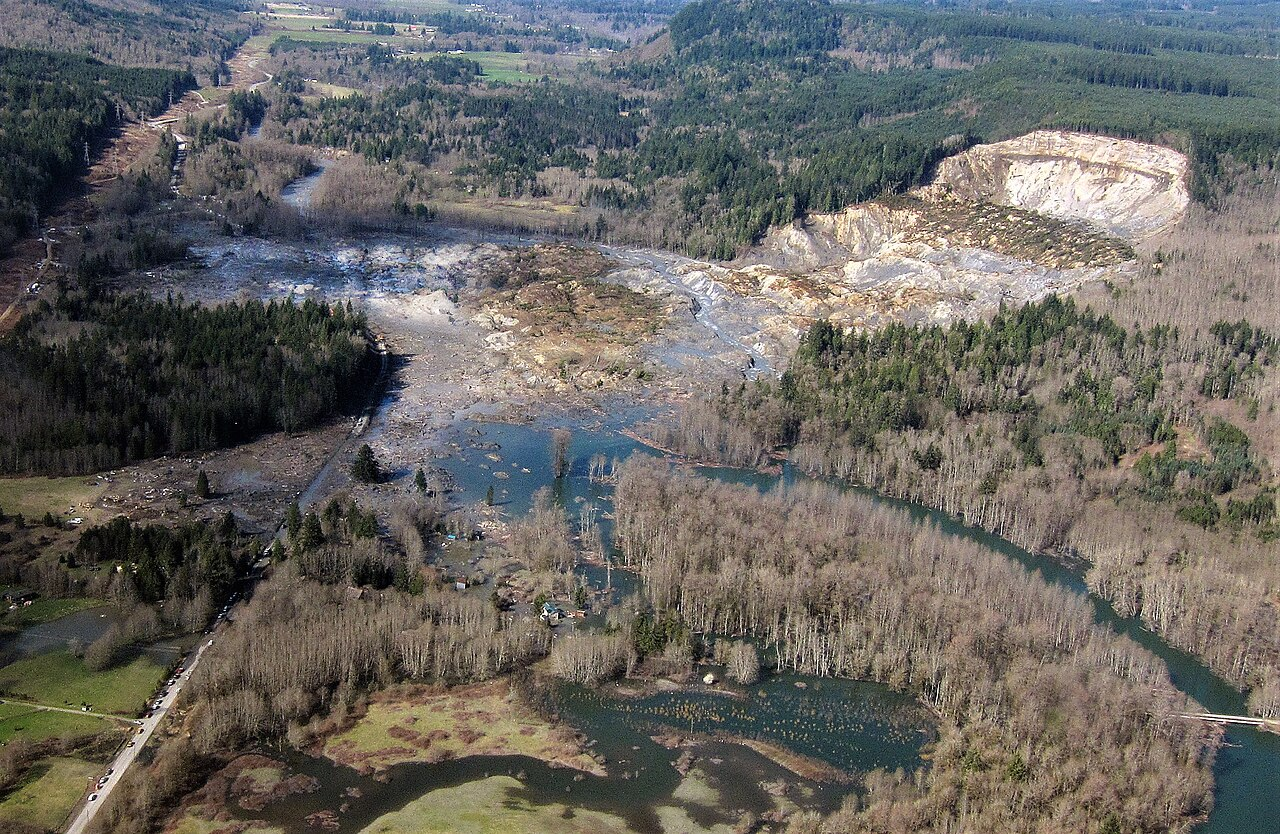
\includegraphics[width=0.6\linewidth]{images/book1/g5-landslide-washington.jpg}

{\small Um grande \omterm{def:g5:natural-hazards:landslide}{deslizamento de terra} no estado de Washington, nos
Estados Unidos, em 2014, visto de um avião. A encosta da direita
desmoronou; a sua \omterm{def:g3:stones-pebbles-sand:sand}{lama} se espalhou por todo o \omterm{def:g1:landscapes-around-us:landform}{vale}, cobriu uma estrada e
bloqueou o \omterm{def:g1:landscapes-around-us:water}{rio}, que inundou a mata \omterm{def:g1:landscapes-around-us:water}{rio} acima. Foto: Mark Reid, U.S.
Geological Survey (domínio público).}\label{fig:g5:natural-hazards:landslide}
% ledger: usgs:oso-aerial
\end{omfigure}

\section{Da ameaça ao desastre}

Uma \omterm{def:g5:natural-hazards:storm}{tempestade} em \omterm{def:g2:water-on-earth:ocean}{alto-mar}, um \omterm{def:g4:volcanoes-earthquakes-first-look:earthquake}{terremoto} num \omterm{def:g5:weather-and-climate:desert}{deserto} vazio, uma \omterm{def:g5:water-shapes-the-land:flood}{inundação}
num \omterm{def:g1:landscapes-around-us:landform}{vale} onde ninguém mora: são \omterm{def:g5:natural-hazards:hazard}{ameaças naturais}, mas não fazem mal a
ninguém. Os mesmos acontecimentos ficam perigosos quando atingem um lugar
onde as pessoas moram.

\begin{definition}[Desastre natural]\label{def:g5:natural-hazards:disaster}
Um \emph{desastre natural}\index{desastre natural} acontece quando uma
\omterm{def:g5:natural-hazards:hazard}{ameaça natural} atinge um lugar onde as pessoas moram e causa grandes
danos: pessoas ficam feridas ou morrem, casas são destruídas, estradas,
água e eletricidade são cortadas.
\end{definition}

\begin{omfigure}
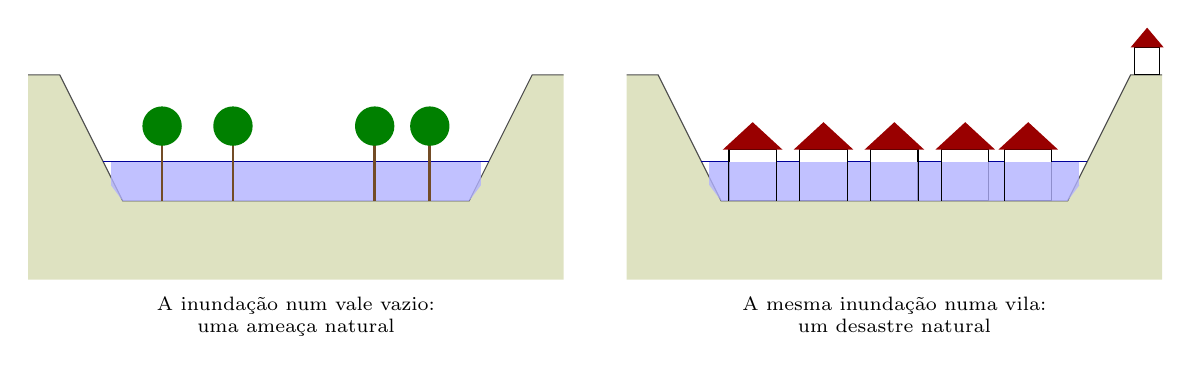
\begin{tikzpicture}[x=1cm, y=1cm, font=\scriptsize]
  \foreach \dx/\title in {0/{A inundação num vale vazio:\\uma ameaça natural},
                          7.6/{A mesma inundação numa vila:\\um desastre natural}} {
    \begin{scope}[xshift=\dx cm]
      % valley sides
      \fill[green!25!brown!30] (0,0) -- (0,2.6) -- (0.4,2.6) -- (1.2,1.0) -- (5.6,1.0)
        -- (6.4,2.6) -- (6.8,2.6) -- (6.8,0) -- cycle;
      \draw[gray!60!black] (0,2.6) -- (0.4,2.6) -- (1.2,1.0) -- (5.6,1.0) -- (6.4,2.6) -- (6.8,2.6);
      % flood water over the whole valley floor
      \fill[blue!30, opacity=0.8] (1.05,1.2) -- (5.75,1.2) -- (5.6,1.0) -- (1.2,1.0) -- cycle;
      \fill[blue!30, opacity=0.8] (1.05,1.2) rectangle (5.75,1.5);
      \draw[blue!60!black] (0.95,1.5) -- (5.85,1.5);
      \node[align=center, anchor=north] at (3.4,-0.1) {\title};
    \end{scope}
  }
  % trees in the empty valley
  \foreach \x in {1.7,2.6,4.4,5.1} {
    \draw[brown!60!black, line width=1pt] (\x,1.0) -- (\x,1.75);
    \fill[green!50!black] (\x,1.95) circle (0.25);
  }
  % houses in the village valley
  \begin{scope}[xshift=7.6cm]
    \foreach \x in {1.6,2.5,3.4,4.3,5.1} {
      \fill[white, draw=black] (\x-0.3,1.0) rectangle (\x+0.3,1.65);
      \fill[red!60!black] (\x-0.38,1.65) -- (\x,2.0) -- (\x+0.38,1.65) -- cycle;
      \fill[blue!30, opacity=0.8] (\x-0.3,1.0) rectangle (\x+0.3,1.5);
    }
    % one house on the high ground, dry
    \fill[white, draw=black] (6.45,2.6) rectangle (6.77,2.95);
    \fill[red!60!black] (6.40,2.95) -- (6.61,3.2) -- (6.82,2.95) -- cycle;
  \end{scope}
\end{tikzpicture}

{\small A mesma \omterm{def:g5:water-shapes-the-land:flood}{inundação} duas vezes. No \omterm{def:g1:landscapes-around-us:landform}{vale} vazio, ela não faz mal a
ninguém; onde uma vila foi construída na \omterm{def:g5:water-shapes-the-land:flood}{planície de inundação}, ela enche
as casas. A casa no terreno alto fica fora da água.}
\end{omfigure}

Não podemos impedir uma \omterm{def:g5:natural-hazards:storm}{tempestade} ou um \omterm{def:g4:volcanoes-earthquakes-first-look:earthquake}{terremoto}. Mas podemos fazer
muito para impedir que uma ameaça vire um desastre: construir longe das
\omterm{def:g5:water-shapes-the-land:flood}{planícies de inundação} e do pé das encostas instáveis, fazer construções
resistentes, vigiar o \omterm{def:g1:watching-the-weather:weather}{tempo} e o chão, avisar as pessoas a tempo e ensinar
a todos o que fazer.

\subsection*{Os alertas}

Os serviços meteorológicos vigiam o céu dia e noite. Quando uma
\omterm{def:g5:natural-hazards:storm}{tempestade}, uma onda de calor ou uma \omterm{def:g5:water-shapes-the-land:flood}{inundação} está chegando, eles mandam
alertas pelo rádio, pela televisão, pelo celular e pela internet. Muitos
países usam cores, da mais calma à mais grave.

\begin{omfigure}
\begin{tikzpicture}[font=\small, wstep/.style={draw=black!60, minimum width=2.6cm,
    minimum height=0.8cm, font=\small\bfseries, rounded corners=2pt}]
  \node[wstep, fill=green!45] (g) at (0,0) {verde};
  \node[wstep, fill=yellow!60] (y) at (0.6,0.95) {amarelo};
  \node[wstep, fill=orange!70] (o) at (1.2,1.9) {laranja};
  \node[wstep, fill=red!65, text=white] (r) at (1.8,2.85) {vermelho};
  \node[anchor=west] at ($(g.east)+(0.3,0)$) {nenhum perigo especial};
  \node[anchor=west] at ($(y.east)+(0.3,0)$) {tenha cuidado, fique informado};
  \node[anchor=west] at ($(o.east)+(0.3,0)$) {esteja preparado: o perigo é provável};
  \node[anchor=west] at ($(r.east)+(0.3,0)$) {grande perigo: aja agora, siga as instruções};
\end{tikzpicture}

{\small Uma escada de cores de alerta. O sentido exato de cada cor muda de
um país para outro: escute sempre as instruções que vêm com o alerta.}
\end{omfigure}

\begin{safety}
\textbf{Numa \omterm{def:g5:natural-hazards:storm}{tempestade}.} Fique dentro de casa, longe das janelas. Não saia
para olhar, e fique longe das árvores, que podem cair, e dos fios
elétricos caídos.

\textbf{Numa \omterm{def:g5:water-shapes-the-land:flood}{inundação}.} Vá para um terreno mais alto ou para um andar de
cima. Nunca atravesse a água de uma enchente a pé, de bicicleta ou de
carro: um pouco de água rápida basta para derrubar você ou arrastar um
carro.

\textbf{Numa onda de calor.} Beba água com frequência, fique na sombra ou
num cômodo fresco nas horas mais quentes, e vá ver como estão os vizinhos
idosos.

\textbf{Num \omterm{def:g4:volcanoes-earthquakes-first-look:earthquake}{terremoto}.} Abaixe-se, proteja-se, segure-se
(\cref{ch:g4:volcanoes-earthquakes-first-look}).

\textbf{Sempre.} Escute os alertas e faça na mesma hora o que os
responsáveis disserem.
\end{safety}

\section{Exercícios}

\begin{exercise}[$\star$]\label{exo:g5:natural-hazards:1}
Só uma \omterm{def:g5:natural-hazards:hazard}{ameaça natural}, ou um \omterm{def:g5:natural-hazards:disaster}{desastre natural}?
\begin{enumerate}
  \item[(a)] Um \omterm{def:g4:volcanoes-earthquakes-first-look:earthquake}{terremoto} sacode um \omterm{def:g5:weather-and-climate:desert}{deserto} vazio.
  \item[(b)] Uma \omterm{def:g5:natural-hazards:storm}{tempestade} arranca o telhado de muitas casas de uma cidade.
  \item[(c)] Um \omterm{def:g5:natural-hazards:landslide}{deslizamento de terra} cai num \omterm{def:g1:landscapes-around-us:landform}{vale} de \omterm{def:g1:landscapes-around-us:landform}{montanha} onde ninguém mora.
  \item[(d)] Um \omterm{def:g1:landscapes-around-us:water}{rio} inunda uma vila e enche as suas casas de água.
\end{enumerate}
\end{exercise}

\begin{exercise}[$\star$]\label{exo:g5:natural-hazards:2}
Classifique estas ameaças em três famílias (do ar, da água, do chão): um
\omterm{def:g5:natural-hazards:landslide}{deslizamento de terra}; uma onda de calor; uma \omterm{def:g5:water-shapes-the-land:flood}{inundação}; uma \omterm{def:g4:volcanoes-earthquakes-first-look:eruption}{erupção}
vulcânica; uma \omterm{def:g5:natural-hazards:storm}{tempestade}; uma \omterm{def:g5:natural-hazards:drought}{seca}; um \omterm{def:g4:volcanoes-earthquakes-first-look:earthquake}{terremoto}.
\end{exercise}

\begin{exercise}[$\star$]\label{exo:g5:natural-hazards:3}
O que é uma \omterm{def:g5:natural-hazards:drought}{seca}? Dê duas maneiras pelas quais uma \omterm{def:g5:natural-hazards:drought}{seca} longa prejudica as pessoas.
\end{exercise}

\begin{exercise}[$\star$]\label{exo:g5:natural-hazards:4}
O rádio anuncia um alerta vermelho de \omterm{def:g5:natural-hazards:storm}{tempestade} para esta noite. Dê três
coisas que a sua família deveria fazer.
\end{exercise}

\begin{exercise}[$\star$]\label{exo:g5:natural-hazards:5}
Uma grande \omterm{def:g5:natural-hazards:storm}{tempestade} que gira, com um olho, se forma sobre um \omterm{def:g2:water-on-earth:ocean}{mar}
tropical quente. Como ela se chama se atingir (a) o \omterm{def:g1:landscapes-around-us:water}{litoral} da Flórida, no
Atlântico Norte; (b) o Japão, no noroeste do Pacífico; (c) o \omterm{def:g1:landscapes-around-us:water}{litoral} da
Índia, no \omterm{def:g2:water-on-earth:ocean}{oceano} Índico?
\end{exercise}

\begin{exercise}[$\star$]\label{exo:g5:natural-hazards:6}
Coloque as quatro cores de alerta em ordem, da mais calma à mais grave. O
que você deve fazer no nível mais grave?
\end{exercise}

\begin{exercise}[$\star\star$]\label{exo:g5:natural-hazards:7}
Observe a foto do \omterm{def:g5:natural-hazards:landslide}{deslizamento de terra} na
página~\pageref{fig:g5:natural-hazards:landslide}. Descreva o que o
deslizamento fez com o \omterm{def:g1:landscapes-around-us:landform}{vale}: com a encosta, com a estrada e com o \omterm{def:g1:landscapes-around-us:water}{rio}. Por
que o terreno \omterm{def:g1:landscapes-around-us:water}{rio} acima agora está embaixo da água?
\end{exercise}

\begin{exercise}[$\star\star$]\label{exo:g5:natural-hazards:8}
Tom diz: ``As \omterm{def:g5:water-shapes-the-land:flood}{inundações} são naturais, então não há nada a fazer.'' Lena
diz: ``Não podemos impedir um \omterm{def:g1:landscapes-around-us:water}{rio} de transbordar, mas podemos impedir que
uma \omterm{def:g5:water-shapes-the-land:flood}{inundação} vire um desastre.'' Quem tem razão? Explique com dois
exemplos.
\end{exercise}

\begin{exercise}[$\star\star$]\label{exo:g5:natural-hazards:9}
Numa região agrícola imaginária, costumam cair cerca de 60 milímetros de
\omterm{def:g4:clouds-rain-snow:precipitation}{chuva} por mês. Durante uma \omterm{def:g5:natural-hazards:drought}{seca}, só caiu um quarto da \omterm{def:g4:clouds-rain-snow:precipitation}{chuva} normal em cada
um de quatro meses.
\begin{enumerate}
  \item[(a)] Quanta \omterm{def:g4:clouds-rain-snow:precipitation}{chuva} costuma cair em quatro meses?
  \item[(b)] Quanto caiu durante a \omterm{def:g5:natural-hazards:drought}{seca}, nos quatro meses?
  \item[(c)] Quanta \omterm{def:g4:clouds-rain-snow:precipitation}{chuva} faltou?
\end{enumerate}
\end{exercise}

\begin{exercise}[$\star\star$]\label{exo:g5:natural-hazards:10}
Uma cidade imaginária tem 1\,200 casas. Um quarto delas fica na \omterm{def:g5:water-shapes-the-land:flood}{planície
de inundação} do seu \omterm{def:g1:landscapes-around-us:water}{rio}.
\begin{enumerate}
  \item[(a)] Quantas casas ficam na \omterm{def:g5:water-shapes-the-land:flood}{planície de inundação}?
  \item[(b)] A cidade ajuda os donos de um terço dessas casas a se mudarem
        para um terreno mais alto. Quantas casas continuam na \omterm{def:g5:water-shapes-the-land:flood}{planície de
        inundação}?
\end{enumerate}
\end{exercise}

\begin{exercise}[$\star\star\star$]\label{exo:g5:natural-hazards:11}
Duas vilas, longe uma da outra, são atingidas por \omterm{def:g5:natural-hazards:storm}{tempestades} da mesma
força na mesma noite. Na primeira, ninguém se fere e os estragos são
pequenos. Na segunda, muitas casas são destruídas. Dê pelo menos três
motivos diferentes que poderiam explicar a diferença.
\end{exercise}
